\documentclass[11pt]{article}
\usepackage{perf}

\begin{document}

    % Set data to be used. Can be reset anywhere.
    \perfset{
    method1 method2 \\
    1     2 \\ % These numbers are the performances on problem 1
    3     4 \\ % Problem 2
    }

    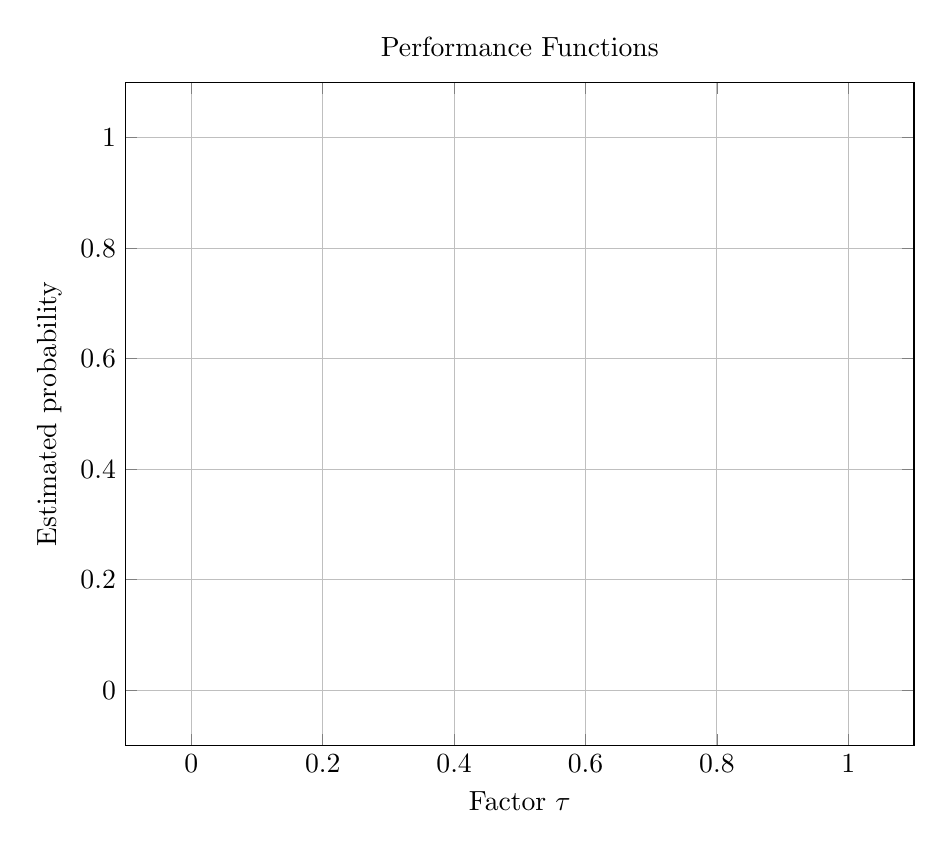
\begin{tikzpicture}
        \begin{axis}[title=Performance Functions,height=10cm,
        legend pos=outer north east,grid=both,no marks, xlabel={Factor $\tau$}, ylabel={Estimated probability}]
            \addprofiles{2}{15} % Param #1: Number of methods to show. Param #2: Upper range for the x axis
            \legend{method1, method2}
        \end{axis}
    \end{tikzpicture}

\end{document}